%% $Id$

%% Copyright (c)  1998-2016
%% by  RWTH-Aachen, Germany
%% Some rights reserved.

%% This work is licensed under the Creative Commons Attribution-Share
%% Alike 3.0 License. To view a copy of this license, visit
%% http://creativecommons.org/licenses/by-sa/3.0/ or send a letter to
%% Creative Commons, 171 Second Street, Suite 300, San Francisco,
%% California, 94105, USA.

\section{Deployment}

\subsection{Physical project structure}
A project contains a set of files that should be grouped to \emph{sourcefiles}, \emph{resources}, \emph{build files} and \emph{configuration} files.
We emphasize the physical separation of these types of files in order to avoid file cluttering that might confuse novice users or developers.
Figure~\ref{fig:ProjectPhysicalLayout} gives an example of a directory tree for an application project.
\begin{figure}
\begin{verbatim}
<project-dir>
 build\
  built\ [temporary storage, created during compilation]
  msvc8\
  Un*x Makefiles
 configfiles\
  *.ini
 resources\
 src\
\end{verbatim}
\caption{\label{fig:ProjectPhysicalLayout}The physical layout of a project.}
\end{figure}
The following sections will give a brief layout of the depicted folder's content.

\subsection{The \code{build} directory}
The \code{build} directory contains all files that are needed for the project to build.
In case a special build directory needs local files to be created during a compilation run, use a separate folder.
For Win32 Microsoft Visual C++ environments, e.g., we differntiate between \code{msvc6}, \code{msvc7} and \code{msvc8} folders that contain workspaces, solutions and projects, see section~\ref{ssec:visualc}.
For Un*x environments, the folder contains the \code{Makefiles} that are needed for the project to build, see section~\ref{ssec:unix}.
This directory should also contain a folder that holds all temporarily created data during a compiler run, e.g., object files.
All build environments should create a folder called \code{built} and put temporary data in here, in different subfolders.
The idea is to have a single directory that needs to be cleaned in order to remove intermediate files and make a project \emph{distclean}, e.g., before you try to copy it over a slow network share.

\subsection{Building rules}
We only support the Visual C++ environment on Win32, and only a recent version.
On Un*x, we are trying to build the projects using recent \code{make} derivatives, e.g., \code{make, gmake} or the like.

\subsubsection{Microsoft Visual C++}\label{ssec:visualc}
The following section describes the settings needed for the Microsoft Visual C++ 8.1 (Visual Studio 2005 SP1).
The Microsoft compiler creates some temporary data during compilation and when working with the IDE itself.
In order to avoid conflicts with co-existing Microsoft compiler suites, e.g., the Visual C++ 6 (\code{msvc6}) or Visual C++ 7 (\code{msvc7}), we store the solution and project files separate directories.
For most project, only the most recent compiler will have properly working project files.

\paragraph{C++ Compiler settings}
\begin{itemize}
\item \textbf{General options}. 
Setup the output and intermediate directories to place their results in the folder \code{../built}, cp. Figure~\ref{fig:visualc.compiler.general}.
In addition to that, please be sure to reflect the comfiguration that was used for building, e.g., Win32 or x64 (for 32/64bit builds on windows) in the output directories' names.
We recommend to use \code{../built/\$(ConfigurationName).WIN32.vc8}.
\item \textbf{Additional Include files}. 
Please refer to a relative include path when you need additional libraries. 
E.g., the \code{VistaTemplate} project resides on the same level as the \code{Vista} libraries, so add the lines \code{../../Vista} to the input line, cp. Figure~\ref{fig:visualc.compiler.general}. 
Add the lines to the \emph{debug} and \emph{release} configurations.
\item \textbf{Code generation}. 
We try to use the memory model \emph{Multi-threaded \{Debug\} DLL}.
Be sure to select this memory model when building your application, cp. Figure~\ref{fig:visualc.compiler.codegeneration}.
\item \textbf{Disable pre-compiled headers}. 
The Microsoft Visual C++ supports the notion of pre-compiled headers, which is to reduce compile times. 
However, as many problems emerge, especially in networked environments, we prefer to switch it off, cp. Figure~\ref{fig:visualc.compiler.precompiled}.
\item \textbf{Linker general settings}. 
We prefer to have a standardized naming policy. 
The name should reflect the configuration it was built for, cp. Figure~\ref{fig:visualc.linker.general}.
Set it to \code{\$(OutDir)/\$(ProjectName).\$(ConfigurationName).exe}.
\item \textbf{Post build events}.
We recommend to copy the compiled files from the intermediate directory to the main directory. 
For that to work, you can use the \code{Post build events}, that can be found in the project's properties \code{Build events} tab.
For example, use \code{copy \$(OutDir)/\$(TargetFileName) ../..} as a macro to do that.
Please note that it is mandatory to use backslashes for the build events, as it simply calls a DOS script, which usually does not respect the slashed notation.
\end{itemize}

\begin{figure}
\includegraphics[width=\linewidth]{visualc}
\caption{\label{fig:visualc.general}
        \label{fig:visualc.compiler.general}
        \label{fig:visualc.compiler.codegeneration}
        \label{fig:visualc.compiler.precompiled}
        Compiler settings, debug configuration.}
\end{figure}

\begin{figure}
\begin{center}
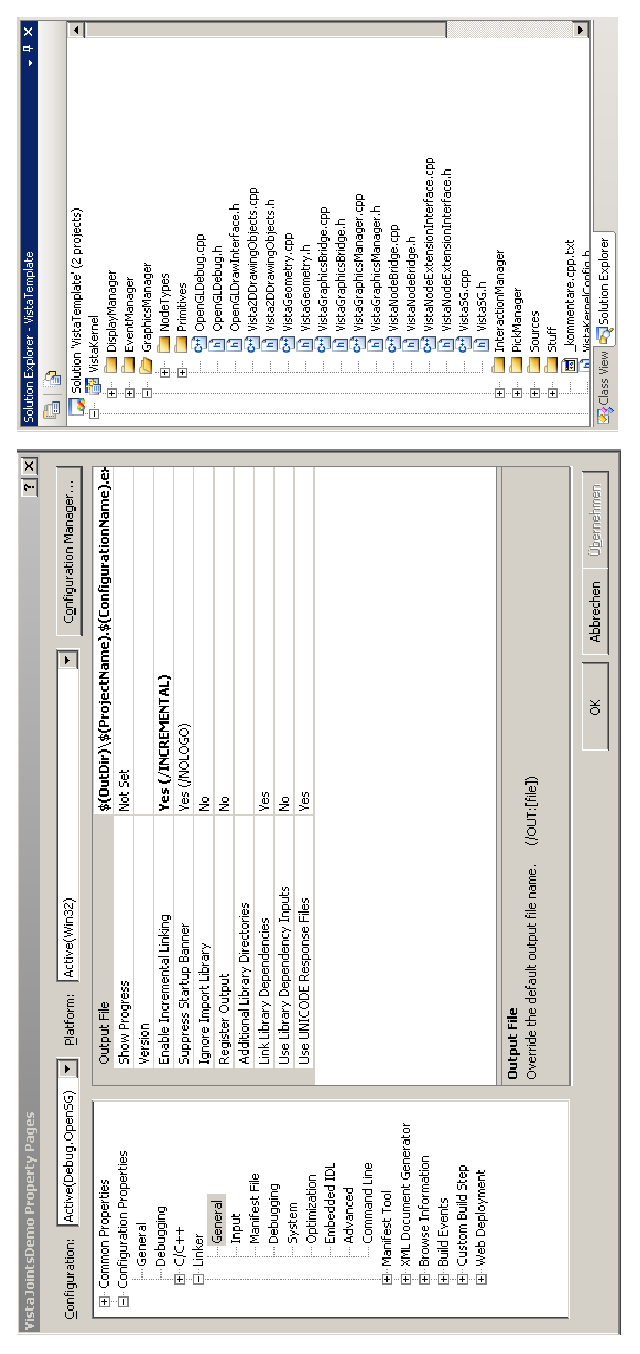
\includegraphics{visualc2}
\end{center}
\caption{\label{fig:visualc.linker.general}
				 \label{fig:visualc_filetree}
         Linker settings and filetree example, debug configuration.}
\end{figure}

For the layout of the directory tree in the projects, we recommend to put headers and source files on the same level, cp. Figure~\ref{fig:visualc_filetree}.
You should provide separate folders, or filters, for resources and configfiles.
Regardless of the physical layout of your folders, you should try to group files using the solution explorer in order to make the navigation in your project as easy as possible.
Try to provide all necessary projects in the solution, but avoid to include projects that you only need during development.
Especially, try to avoid to include the \code{ViSTA} core libs in your application solution.

\paragraph{Common Release Options for Win32 builds}

Following excerpts from the MSDN we recommend the settings for win32 builds, as depicted in the following table.

\begin{tabular}{|l|p{10cm}|}
\multicolumn{2}{c}{\textbf{Compile time options for the msvc}}\\\hline
\textbf{Platform} & \textbf{Options}  \\\hline
P3+, AthlonXP+ & /arch:SSE /G6 /O2\\\hline
P4+, Athlon64, AthlonFX & /arch:SSE2, /G7, /O2\\\hline
\end{tabular}

\newpage
\subsubsection{Using \code{make} on Un*x}\label{ssec:unix}
There is a uniform Makefile structure which is used in all \code{ViSTA} core and add-on libraries.
It is encouraged to adapt to this structure for all projects based on \code{ViSTA}.
It consists of the following essential components:

\begin{itemize}
  \item user configurable files containing per-project information:
    \begin{itemize}
    \item \code{build/Makefile.project} - project Makefile, contains project related definitions which are common for all platforms.
    \item \code{build/Makefile.\$(R\_OSTYPE)} - contains platform-specific definitions. One should exist for each supported platform (\code{SUNOS}, \code{LINUX}, ...).
    \item \code{build/Makefile.objects} - contains the names of all object files which constitute the library/executable to be built.
    \end{itemize}
    
  \item files (normally) not to be configured by the user, containing static build information
    \begin{itemize}
    \item \code{Makefile} - top-level Makefile, contains only the target definitions and references/includes the other build components.
    \item \code{Vista/VistaMakefiles/Makefile.build} - Contains the generic build rules and those for dependency generation.
    \item \code{Vista/VistaMakefiles/Makefile.MODULE} - ``Module-Makefiles'', allow comfortable addition of (third-party) libraries to a project or library.
    \item \code{.bashrc}, \code{.zshrc}, \code{.profile} or similar - The environment has to contain some definitions for the other build components to work.
    \end{itemize}
\end{itemize}

The build process works the following way. One of the top-level targets (described later in detail) is called from the command line using (preferrably GNU) \code{make}.
Depending on the target, a new sub-make using \code{Makefile.project} is called with the make variables \code{MODE} and \code{TOOLKIT} set to the respective values.
\code{Makefile.project} sets project-wide variables and includes \code{Makefile.\$(R\_OSTYPE)} at the beginning, where the platform-specific variables are set.
\code{Makefile.project} then includes \code{Makefile.COMMON} and the module-Makefiles at the end, and finally includes \code{Makefile.build}.

The user-configurable files in detail:
\begin{itemize}
  \item \code{Makefile.project}:

    Variables:\\
    
\begin{longtable}{|l|p{12.75cm}|}
  \hline
  \code{TYPE} &  The type of project. 
  Determines the naming scheme of the output file. 
  Possible values: \code{BIN} for binary/executable, \code{LIB} for (currently only static) library.\\\hline
  \code{OUTDIR} & The output directory. 
  The linked executable/library is copied into this folder after compilation.\\\hline
  \code{BUILTDIR} & The temporary files directory. 
  Object files created during the build are placed in here. Typically \code{build/built}. \\\hline
  \code{SUBDIRS} & In case directories have to be created for the build to work, they can be placed here to be recreated e.g. after a \code{make clean}. \\\hline
  \code{SRCDIRS} & All Folders containing source files corresponding to the object files listed in \code{Makefile.objects}.\\\hline
\end{longtable}

    At the end of \code{Makefile.project}, the module-Makefiles are included. 
    The first lines after the variable definitions should always be:

    \code{VISTA\_ROOT ?= /path/to/your/Vista} \\
    \code{include \$(VISTA\_ROOT)/VistaMakefiles/Makefile.COMMON}

    Then, makefile-modules may be included using the same make include syntax:

    \code{include \$(VISTA\_ROOT)/VistaMakefiles/Makefile.MODULE}

    \item \code{Makefile.\$(R\_OSTYPE)}:

      \begin{longtable}{|l|p{7cm}|}
      \hline
      \code{SYSTEM} & The system type, should correspond to R\_OSTYPE. \\\hline
      \code{BASEDIRECTORY} & The base directory for all libraries adhering to the directory structure described in \ref{dir_struct}, i.e. the \code{vrsoftware} or \code{vrsw} directories. \\\hline
      \code{ADDOBJS} & Platform specific object files which do not go into \code{Makefile.objects}. \\\hline
      \code{ADDLIBDIRS} & References to library directories not included via makefile-modules. 
                          In the form \code{-Llibdir}. \\\hline
      \code{ADDLIBS} & References to libraries not included via makefile-modules. In the form \code{-llib}. \\\hline
      \code{ADDINCLUDES} & References to include folders not included via makefile-modules. 
                           In the form \code{-Iincludedir}. \\\hline
      \code{COMPILER} & The compiler executable. Should be \code{\$\{CXX\}} per default. \\\hline
      \code{LINKER} & The linker executable. Should be \code{\$\{CXX\}} per default for executables, possibly \code{ar} for static libraries. \\\hline
      \code{CFLAGS\_\{DEBUG,RELEASE\}} & The compiler flags passed during compilation, for debug or release mode respectively. \\\hline
      \code{LFLAGS\_\{DEBUG,RELEASE\}} & The linker flags passed during compilation.\\\hline
      \code{ARCHFLAGS\_\$(VISTA\_HWARCH)} & Architecture specific compiler flags, as e.g. \code{-m32} for i386 32bit. \\\hline
      \code{DEPFLAG} & Compiler-specific flag for dependency generation, e.g. \code{-MM} for gcc.\\\hline
      \end{longtable}

    \item \code{Makefile.objects}:

      \begin{longtable}{|l|p{10cm}|}
      \hline
      \code{OBJS} & The list of object files. \\\hline
      \code{OBJS\_WTK} & The list of object files contained only in the WTK build. \\\hline
      \code{OBJS\_OSG} & The list of object files contained only in the OpenSG build. \\\hline
      \end{longtable}

      The definition for each of the variables has to be in the following form (regardless of the folder where the corresponding source file resides):

      \ttfamily
	OBJS = \${OBJDIR}/object1.o $\backslash$ \\
	\hspace*{4em}\${OBJDIR}/object2.o
      \rmfamily
\end{itemize}

Commonly not user-configured files roughly explained:
\begin{itemize}
  \item \code{build/Makefile}:

    Defines the availabe make targets. 
    It should always include \code{debug}, \code{release} and \code{clean}. 
    These typically refer to the corresponding toolkit specific target, for example \code{debug\_osg} and \code{debug\_wtk}. 
    For projects which do not use VistaKernel for graphical output at all, there might be a \code{*\_notk} target available.
    \code{Makefile} then starts a new sub-make process using \code{Makefile.project}, and passes the corresponding values for \code{MODE} and \code{TOOLKIT}.

  \item \code{Vista/VistaMakefiles/Makefile.build}

    Contains the (pretty unreadable) generic build rules where all variable definitions are finally transformed into compiler/linker commands.
    You should not need to edit this file ever, if so please contact their original author if possible.

  \item \code{Vista/VistaMakefiles/Makefile.MODULE}

    These Makefiles constitute "subsystem-modules" which can easily be included in a build-process using 

    \code{include \$(VISTA\_ROOT)/VistaMakefiles/Makefile.MODULE} 

    at the end of \code{Makefile.project}.    
    They all have a very similar structure which is explained below. The module-specific libraries and includes are simply appended to the global variables. 
    Thus, the order in which they are included is important (e.g. \code{Makefile.VISTA} has to be included before \code{Makefile.OSG} because the \code{ViSTA} libraries depend on OpenSG). 
    In \code{Makefile.COMMON}, common things like determining the application's name and including the object files are performed. 
    It always has to be included first, in every project, for the build structure to work properly. 
    If not specified explicitly, the paths are selected relative to \code{\$(BASEDIRECTORY)}, custom roots for specific modules can be set using \code{MODULE\_ROOT=dir} before the include directive.
    Have a look at the contents of \code{Vista/VistaMakefiles} to find out which modules currently exists, and feel free to add new ones, adhering to the following format (substitute module with the name of the actual module):

    \ttfamily
\begin{verbatim}
#=====================
#== MODULE SETTINGS ==
#=====================

MODULE_ROOT  ?= ${BASEDIRECTORY}/moduledir/$(SYSTEM)

MODULEINCL    = -I$(MODULE_ROOT)/include

MODULELIBDIR_RELEASE	= -L$(MODULE_ROOT)/lib/debug
MODULELIBDIR_DEBUG  	= -L${MODULE_ROOT}/lib/release
MODULELIBDIR		= $(MODULELIBDIR_$(MODE))

MODULELIBS		= -llibname

LIBDIRS  += $(MODULELIBDIR)
LIBS     += $(MODULELIBS)
INCLUDES += $(MODULEINCL)
\end{verbatim}
    \rmfamily

  \item \code{.bashrc, .zshrc, .profile, ...}
    
    Some Environment variables have to be set in order to make the build process work correctly: \\

    \begin{longtable}{|l|p{10.00cm}|}
      \hline
      \code{CXX} & The C++ compiler \\\hline
      \code{VISTA\_HWARCH} & The hardware architecture. possibles values are \code{IA32}, \code{IA64}, \code{OP32}, \code{OP64}, \code{SPARC32}, \code{SPARC64}, \code{MIPS32} and \code{MIPS64}. \\\hline
      \code{VRSOFTWARE} & Location of the central ViSTA software repository. \\\hline
      \code{R\_OSTYPE} & Either \code{LINUX}, \code{SUNOS}, \code{IRIX} or \code{HP-UX}, typically set by the OS itself. \\\hline
      \code{CFLAGS/LFLAGS} & May also be set from the environment. 
      If set, \bfseries only \mdseries those, and not the C/LFLAGS from Makefile.\$(SYSTEM) will be taken. 
      Thus, for normal operation, \bfseries do not set CFLAGS or LFLAGS in your environment!\mdseries \\\hline
    \end{longtable}
\end{itemize}




\subsection{The \code{configfiles} directory}
This directory should hold all initialization files that are needed to run the application or associated tools.
Note that this folder can be used to store auxiliary files, such as data or timing files that may be read by your application.
However, it is possible that many files are needed for a proper configuration of your application, so this folder helps to avoid file cluttering in the main directory.
The \code{vista.ini} is a popular example to store in this directory.

\subsection{The \code{resources} directory}
The \code{resources} folder is used to store additional resources that can not really be classified.
As an example, think of bitmap graphics or model files that are not directly needed in the application but are used as sources for application used resources.
It is most useful to collect resource files during the development, as they allow to rebuild some structures in case they are lost.
In addition to this, this folder can hold auxiliary files such as code templates.
It can be used to store some files needed for documentation, e.g., Doxygen configuration files.
It should, however, not be used to store documentation files themselves.


\subsection{The \code{src} directory}
This directory contains source and header files, and may even contain some other source file subfolders.
For \textit{applications} this is the only source related folder.
For \textit{libraries} this strategy is recommended, too.
We do not employ the usage of different \code{src} and \code{include} directories, as this strategy is not very practicable on Microsoft Windows development environments.

\subsection{The \code{project} directory}
The directory itself can contain readme files, the binaries that are produced by compilation and other runtime resources, such as scripts, models or bitmap graphics.

\section{External libraries and packages}
Every software code resource that is used, which is not produced in-house is called \emph{external} software, or \emph{3rd party} software.
It is a must to distinguish between in house produced code and 3rd party software.

\subsection{Legal issues}
For the complete development, is is absolutely mandatory to respect the legal constraints that 3rd party software is shipped with.
In general, for ViSTA libraries, only software code that does not force us to deliver source code to anybody is to be used.
This means especially, that under almost no circumstances GPL or similiar licensed software may be used for the ViSTA core libraries, and even add-on libraries.
This rule is not necessarily enforced for applications.
The latter sentence means that project maintainers and application developers are free to use any software component they like, as long as they do not incorporate commercial or GPLed software to the ViSTA core libraries.

\subsection{Deployment}
In order to ease the usage of 3rd party libraries, we enforce a set of rules that have to be respected when deploying these libraries to the ViSTA users.
In general, it is wanted to stick to the 3rd party deployment process as close as possible, that means that we do not necessarily enforce naming changes, e.g. to libraries.
The idea is that it should be the most natural process to update to current versions of 3rd party software, but to ease the usage for ViSTA users.
In general, think carefully about updating 3rd party libraries when it is not an absolute must.
As a genereal rule of thumb, \textbf{never change a running system}.
Again, if you do not encounter trouble with a 3rd party implementation (either performance, stability or security), do not update without a deeper reason.
In general, think about the portability of 3rd party libraries before incorporating them to your project.
Do only consider those that are running the same platforms as ViSTA does, when applying them to ViSTA core or add-on libraries.


\subsubsection{Building 3rd party libraries from source}
\paragraph{Unix}
On Unix, more precisely under the autoconf/automake building environment or similiar, build the 3rd party code from scratch for every platform.
When done, save all dependent files (e.g., headers and source files) before building for a different platform.
Some build environments apply changes to headers and source files (e.g., during \code{configure}) and it is a general \emph{no-go} to use, e.g., the same headers for LINUX and SUNOS builds.
\begin{itemize}
\item Try to note the build options, either in a seperate \code{README.txt} or, if the building environment allows this, in a build specific output format.
\item Try to build unix libraries with as less dependencies as possible, e.g., avoid the inclusion of rarely supported image formats, if they are not really needed.
When in doubt, specifiy your build strategy for each platform in a dedicated file (you might need the information after a long time, when trying to update).
\item Try to build libraries as shared and static link objects, if this is supported by the library.
\item Try to use the compiler that is specified for your platform, especially when building C++ libraries.
Do, at all costs, note the compiler type and version you used when building the library.
\end{itemize}
It is good practice to provide a module makefile for 3rd party libraries that allow users to compile and link with the 3rd party libraries quickly.

\paragraph{Windows}
We do only support the Microsoft Visual C++ environment.
Here, build all libraries as \emph{multithreaded DLL} configurations (for static and DLL libraries).
Try to provide the build files you used to build the projects (e.g., vcproj and sln files).

\subsection{Deploying libraries}
This section deals with the job of deploying your builds to users of your or ViSTA libraries.
It is important to see the difference between users and developers of your work.
For users, it is generally not really important, which revision to use, while it can be crucial for developers, as some features might be supported and some are not.

\paragraph{Names and Revisions}
\label{dir_struct}
In general, simple users should have the knowledge about which libraries to use, and a very basic knowledge about the revision which is to be used.
As a consequence, it is good practice to consider the level of generality for 3rd party libraries.

As an example, imagine that you use the FOX toolkit for 2D GUI applications.
FOX comes itself in more than one revision, the 1.4 (called \textit{old stable}), the 1.6 (called \textit{stable}) and the 1.7 (called \textit{unstable} or \textit{release}).
In addition to that, FOX uses a third level of versioning, the \textit{patch level}.
In that sense, the current FOX 1.4 is revisioned as 1.4.35.
In general, as a project maintainer, you should decide which is your \textit{current} version you work with.
In that sense, you tell your user ''I use FOX for my 2D GUI, currently the 1.4, old stable''.
Usually, users do not care for the patch revision.

A good deployment on the general software network share (on a unix home) for that example is as follows.

\begin{verbatim}
|...
|- fox -> fox-1.4.35         // <- indicates the ''default''
|- fox-1.4 -> fox-1.4.35     // <- special link 
|- fox-1.4.35                // <- real source
|  |- LINUX
|  |  |- include
|  |  |- libs
|  |  |- source
|  |  |  |- <original lib>
|  |- SUNOS
|  |  |- include
|  |  |- libs
|  |  |- source
|  |  |  |- <original lib>
|  |- WIN32
|  |  |- include
|  |  |- libs
|  |  |- source
|  |  |  |- <original lib>
|- fox-1.6 -> fox-1.6.20
|- fox-1.6.20
|  |- LINUX
|  |  |- include
|  |  |- libs
|  |  |- source
|  |  |  |- <original lib>
|  |- SUNOS
|  |  |- include
|  |  |- libs
|  |  |- source
|  |  |  |- <original lib>
|  |- WIN32
|  |  |- include
|  |  |- libs
|  |  |- source
|  |  |  |- <original lib>
| ...
\end{verbatim}
The above depicted example indicates that normal users should use ''fox'' as their base, not really caring which specific version it is.
Some users that use special code need to know at least the major and minor revision, without the patch level.
For those, a direct link is provided, and patch levels can transparently be replaced.
The original source code should be available for debugging purposes, but should only be read-writeable by the project maintainer or the vrsw user on our unix home.
It should be mentioned that the provided source code is not to be patched in the public space, but in a private space and when working, the 3rd party library is to be redistributed.
\paragraph{Deploying C libraries}
C libraries are not as sensitive to compiler changes as C++ libraries are.
For that reason, it is ok to place C libraries as they are compiled to the 3rd party deployment \code{libs} directory.
For C++ libraries, a number of different binaries can exist concurrently, e.g, compiled for the g++ 3.x or gcc 4.x branch of compilers.
If that is the case, create special directories beneath the \code{libs} directory of the 3rd party library and use a proper naming scheme to adress the build.
The same accounts for 32bit and 64bit builds (although we do not enforce 64bit builds right now).
\begin{verbatim}
|...
|- fox -> fox-1.4.35         // <- indicates the ''default''
|- fox-1.4 -> fox-1.4.35     // <- special link 
|- fox-1.4.35                // <- real source
|  |- LINUX -> LINUX_GCC3.2_IA32
|  |- LINUX_GCC3.2_IA32
|  |  |- include
|  |  |- libs
|  |  |- source
|  |  |  |- <original lib>
|  |- LINUX_GCC4.0_IA32
|  |  |- include
|  |  |- libs
|  |  |- source
|  |  |  |- <original lib>
|...
\end{verbatim}

\paragraph{Storage}
We employ a public software network share that enables users to transparently link their application to prebuilt libraries.
Please be aware that changes on this public repository should be done with care, as some projects may rely on a static layout.

Currently, the software network share resides at the following locations.
\begin{itemize}
\item Unix: \code{/home/vrsw}
%\item Windows://vfsc4.rz.rwth-aachen.de/vrsoftware
\item Windows: \code{$\backslash$$\backslash$cifs.rz.rwth-aachen.de$\backslash$cluster$\backslash$project$\backslash$vrsoftware}
\end{itemize}
In order to put the 3rd party libraries to the shared network space, please be aware of read and write access to those files.
For this reason, a special user in the unix domain exists, which is called \emph{vrsw}.
Do only place libraries to the shared space under this user's access rights and use the av00 group for group access.

